\documentclass[11pt,a4paper]{article}

\usepackage[utf8]{inputenc}
\usepackage[T1]{fontenc}
\usepackage{lmodern}
\usepackage[margin=2.5cm]{geometry}
\usepackage{amsmath,amssymb}
\usepackage{graphicx}
\usepackage{booktabs}
\usepackage{caption}
\usepackage[authoryear,round]{natbib}
\usepackage[hidelinks]{hyperref}

\graphicspath{{figures/}}

\title{Credit Valuation Adjustment of an Interest Rate Swap\\
\large Exposure, Collateral, Netting and Wrong-Way Risk under a Calibrated Hull--White Model}
\author{Andreas Kyrlakis\\
\small MSc in Finance, HEC Lausanne (University of Lausanne)}
\date{November 2026}

\begin{document}
\maketitle

\begin{abstract}
\noindent
When a bank trades an uncollateralised derivative with a corporate client, it is exposed to the client's default whenever the trade has a positive value. The credit valuation adjustment (CVA) is the price of this risk. This paper computes the CVA of a 10-year, USD 100 million payer interest rate swap with a BBB counterparty, using only free market data from 17 November 2026. The US Treasury curve is bootstrapped from constant-maturity par yields, and a one-factor Hull--White model is fitted exactly to it, with mean reversion $a=0.012$ and volatility $\sigma=91$ bp estimated from three years of zero-yield volatility. With 20{,}000 exactly simulated paths, the expected exposure peaks at USD 4.6 million and the 97.5\% potential future exposure at USD 19.1 million, both after 4.5 years. With a hazard rate implied by the BBB option-adjusted spread (1.15\%) and a 60\% loss given default, the CVA is USD 262{,}000 (standard error 935), or 3.4 bp a year on the fixed rate. The Monte Carlo is validated against the Jamshidian swaption formula at every reset date (maximum relative error 1.5\%). A two-way collateral agreement with a zero threshold and a 10-business-day margin period of risk removes 90\% of the CVA; netting the swap with an offsetting 5-year receiver removes 35\% of the combined CVA. Finally, when the counterparty's default intensity is positively correlated with interest rates (wrong-way risk), the CVA rises by 55\% at a correlation of 0.6 with the default probabilities unchanged.
\end{abstract}

\section{Introduction}

Since the 2008 crisis, the fair value of an over-the-counter derivative includes an adjustment for the default risk of the counterparty \citep{gregory2020}. Under IFRS~13 banks book a CVA in their accounts, and under Basel~III they hold capital against its variability \citep{basel2017}. The CVA desk of a bank charges this cost to the trading desk when a new trade is booked, and hedges it.

The CVA of a trade combines three ingredients: how much the bank could lose at each future date (the \emph{exposure}), how likely the counterparty is to default at that date, and how much would be lost after default. The exposure is the hard part: it depends on the future value of the trade, so it requires a model of the underlying market factors. For interest rate swaps, the standard tool is a short-rate model such as \citet{hullwhite1990}, simulated by Monte Carlo \citep{pykhtin2007,brigo2013}.

This paper builds this computation from end to end for a single, standard trade: the bank pays a fixed rate on a 10-year USD 100 million interest rate swap with a corporate client rated BBB. We then answer four questions that a CVA desk faces every day:
\begin{enumerate}
  \item What are the exposure profiles and the CVA of the trade, and how sure are we of the number?
  \item How much does a collateral agreement (CSA) reduce the CVA, depending on its threshold and on the margin period of risk?
  \item How much does netting with other trades of the same client help?
  \item How much does the answer change if default risk and interest rates move together (wrong-way risk)?
\end{enumerate}

\section{Data}

All data are free, need no account, and are downloaded again by the code from FRED (Federal Reserve Bank of St. Louis). The valuation date is 17 November 2026, the last day with a complete Treasury curve at download time (19 November 2026).

\begin{itemize}
  \item \textbf{Interest rates.} Daily US Treasury constant-maturity par yields (H.15 release) at 11 maturities from 1 month to 30 years, since January 2016. On the valuation date they range from 4.09\% (1 month) to 5.10\% (10 years) and 5.46\% (30 years). The overnight SOFR rate (3.92\%) is kept for reference only.
  \item \textbf{Credit.} The ICE BofA US corporate option-adjusted spreads over Treasuries for the BBB index (1.15\%, used for the counterparty) and the A index (0.76\%, used for the bank itself). FRED makes only the last three years of these series available.
\end{itemize}

A real USD swap is priced on the SOFR curve, but SOFR swap rates are not available for free. We therefore price the swap on the Treasury curve, with a single curve for projecting the floating rate and for discounting. This changes the level of the par swap rate (it equals the 10-year Treasury par yield, 5.10\%), but has little effect on the shape of the exposure, which is driven by rate volatility. We come back to this limitation in Section~\ref{sec:limits}.

\section{Method}

\subsection{Zero curve}

Bills (1, 3 and 6 months) quote a bond-equivalent yield, which we read as a zero rate with semi-annual compounding: $P(0,T) = (1+y/2)^{-2T}$. From one year on, the quoted yield is the coupon $c$ of a bond priced at par that pays $c/2$ every six months. Par yields are interpolated linearly on a six-month grid up to 30 years and discount factors are bootstrapped one date at a time:
\begin{equation}
P(0,T_n) = \frac{1 - \tfrac{c_n}{2}\sum_{i<n} P(0,T_i)}{1+\tfrac{c_n}{2}} .
\end{equation}
Between nodes, $\log P(0,t)$ is interpolated linearly (piecewise flat forward rates). The bootstrapped curve reprices all eight par bonds to within $10^{-16}$. Figure~\ref{fig:curve} shows the curve: the zero rate rises from 4.3\% at three months to 5.6\% at 20 years.

\begin{figure}[h]
\centering
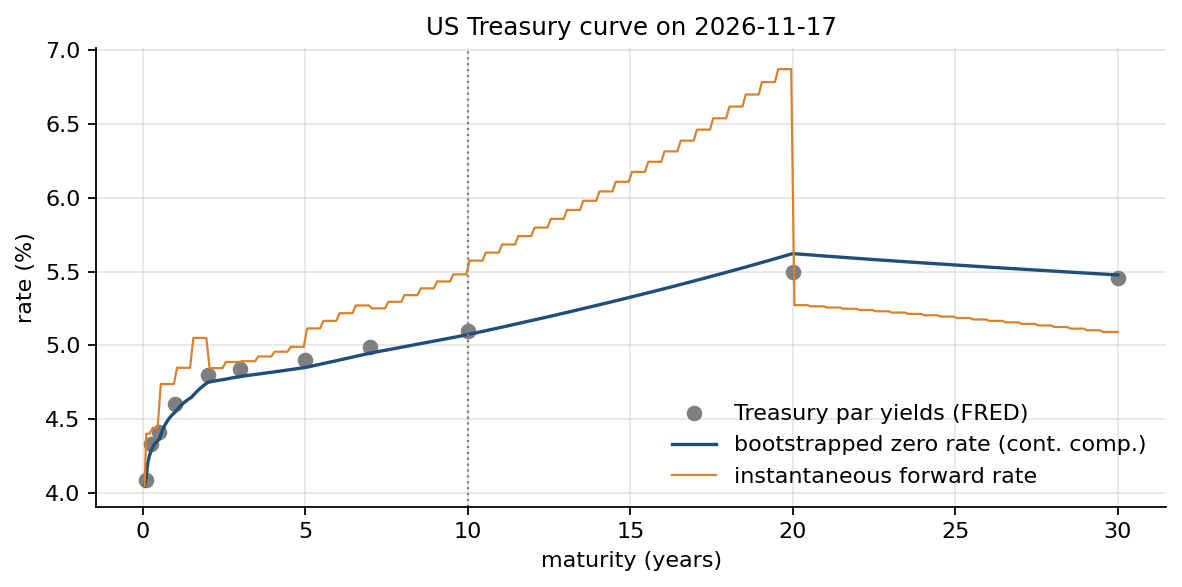
\includegraphics[width=0.85\textwidth]{fig1_curve.png}
\caption{US Treasury par yields on 17 November 2026, bootstrapped zero rates and instantaneous forward rates.}
\label{fig:curve}
\end{figure}

\subsection{Hull--White model}

We use the one-factor Hull--White model in the form of \citet[Section 3.8]{brigo2006}:
\begin{equation}
r(t) = x(t) + \varphi(t), \qquad dx(t) = -a\,x(t)\,dt + \sigma\,dW(t), \quad x(0)=0,
\end{equation}
where $\varphi$ is the deterministic function that makes the model reproduce today's discount factors exactly. Zero-coupon bond prices are then
\begin{equation}
P(t,T) = \frac{P(0,T)}{P(0,t)} \exp\!\Big(\tfrac12\big[V(t,T)-V(0,T)+V(0,t)\big] - B(t,T)\,x(t)\Big),
\label{eq:bond}
\end{equation}
with $B(t,T) = (1-e^{-a(T-t)})/a$ and $V(t,T) = \frac{\sigma^2}{a^2}\big[T-t+\frac{2}{a}e^{-a(T-t)} - \frac{1}{2a}e^{-2a(T-t)} - \frac{3}{2a}\big]$. This form needs only the discount factors, not the derivative of the forward curve.

\paragraph{Exact simulation.} The pair $\big(x(t), I(t)=\int_0^t x(s)\,ds\big)$ is jointly Gaussian, with known transition mean and covariance on any time step. We simulate it exactly, so the bank-account deflator
\begin{equation}
D(t) = e^{-\int_0^t r(s)ds} = P(0,t)\, e^{-\frac12 V(0,t) - I(t)}
\end{equation}
has no time-discretisation bias, and $\mathbb{E}[D(t)] = P(0,t)$ holds exactly in the model. We use antithetic variates.

\paragraph{Calibration.} A trading desk calibrates $a$ and $\sigma$ to swaption implied volatilities, which are not available for free. We use the historical alternative: in the model, the normal volatility of the $\tau$-year zero yield is $\sigma B(0,\tau)/\tau$, which decreases with maturity at a speed set by $a$. We bootstrap the zero curve on each of the last 747 trading days (20 November 2023 to 17 November 2026), compute the annualised standard deviation of the daily changes of the 1- to 30-year zero yields, and fit $(a,\sigma)$ by least squares. The 1-year volatility (65 bp) sits below a hump (90 bp at 2--5 years) that a one-factor model cannot produce, because the front end is anchored by Federal Reserve policy; we fit the 2- to 30-year points. The fit gives $a=0.0118$ and $\sigma=91.0$ bp per year, with a root mean squared error of 1.8 bp (Figure~\ref{fig:volfit}).

\begin{figure}[h]
\centering
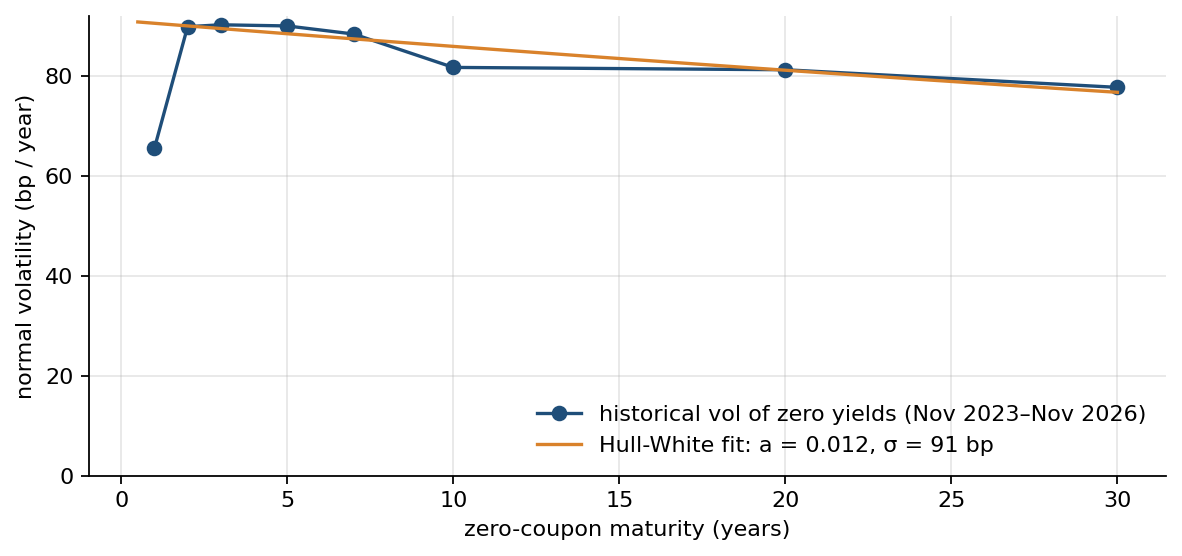
\includegraphics[width=0.85\textwidth]{fig2_yield_vol_fit.png}
\caption{Historical normal volatility of zero yields (daily changes, annualised) and the Hull--White fit on the 2- to 30-year maturities.}
\label{fig:volfit}
\end{figure}

\subsection{Swap valuation on each path}

The bank pays a fixed rate $K$ and receives the floating rate on USD 100 million for 10 years; both legs pay semi-annually with accrual $\delta=0.5$. $K = 5.100\%$ is the par rate, so the swap is worth zero today. At a future date $t$, with remaining payment dates $T_j > t$, the value of the payer swap is
\begin{equation}
V(t) = N\Big[F(t) - P(t,T_n)\Big] - N K \delta \sum_{j} P(t,T_j),
\end{equation}
where $F(t) = P(t,T_{j_0})/P(T_{j_0}-\delta,T_{j_0})$ if the current coupon has already been fixed at $T_{j_0}-\delta$, and $F(t)=1$ on a fixing date. Every bond price comes from equation~\eqref{eq:bond}, so the valuation on each path is exact. The fixing $P(T_{j_0}-\delta, T_{j_0})$ is stored on each path when the simulation reaches the reset date; the grid therefore contains all reset dates. Values are taken just after any payment due at $t$.

We use a grid with a step of two weeks (260 steps over 10 years, about 10 business days per step) and 20{,}000 paths.

\subsection{Exposure measures and CVA}

With $V(t)$ the value of the netting set for the bank, we compute at every grid date:
\begin{align*}
\text{EE}(t) &= \mathbb{E}[\max(V(t),0)], &\quad \text{EE}^*(t) &= \mathbb{E}[D(t)\max(V(t),0)], \\
\text{PFE}(t) &= q_{97.5\%}\big(\max(V(t),0)\big), &\quad \text{ENE}^*(t) &= \mathbb{E}[D(t)\max(-V(t),0)],
\end{align*}
and the expected positive exposure $\text{EPE} = \frac{1}{T}\int_0^T \text{EE}(t)\,dt$ (and the Basel effective EPE over one year, which uses the non-decreasing envelope of EE).

The counterparty's default time has a flat hazard rate $\lambda$ obtained from its credit spread $s$ by the credit triangle, $\lambda = s/\text{LGD}$. With $s=1.15\%$ and $\text{LGD}=60\%$, $\lambda = 1.92\%$ a year and the 10-year default probability is 17.4\%. Assuming independence between default and rates, the unilateral CVA is
\begin{equation}
\text{CVA} = \text{LGD} \sum_{i} \overline{\text{EE}}^*_i \big[S(t_{i-1}) - S(t_i)\big], \qquad S(t) = e^{-\lambda t},
\end{equation}
where $\overline{\text{EE}}^*_i$ is the average of $\text{EE}^*$ at both ends of the interval. The DVA is the same formula applied to $\text{ENE}^*$ with the bank's own spread (A index, 0.76\%, $\lambda=1.27\%$). In the bilateral (first-to-default) version, each term of the CVA is multiplied by the survival probability of the bank, and vice versa \citep{brigo2013}.

\subsection{Collateral, netting and wrong-way risk}

\paragraph{Collateral.} Under a two-way CSA with threshold $H$, the collateral held at $t$ is the amount called at the last date before the margin period of risk (MPR) $\Delta$, when the counterparty stopped posting:
\begin{equation}
C(t) = \big(V(t-\Delta) - H\big)^+ - \big(-V(t-\Delta) - H\big)^+ ,
\end{equation}
and the collateralised exposure is $\max(V(t)-C(t),0)$ \citep{gregory2020}. We use MPRs of 0, 10 and 20 business days (0, 1 and 2 grid steps).

\paragraph{Netting.} The values of all trades in a netting set are added on each path before taking the positive part. We value the 10-year payer swap together with either an offsetting 5-year receiver swap or a 5-year payer swap, both at par, on the same paths.

\paragraph{Wrong-way risk.} We let the default intensity of the counterparty be stochastic, $\lambda(t) = \phi(t)\,e^{Y(t)}$, where $Y$ is an Ornstein--Uhlenbeck process, $dY = -\kappa Y dt + \eta\, dW_Y$, whose shocks have correlation $\rho$ with the shocks of the short rate. For each $\rho$, the function $\phi(t)$ is recalibrated on the grid so that the average simulated survival curve equals the market curve $e^{-\lambda t}$ (to within $10^{-8}$). Only the dependence between exposure and default changes, not the default probabilities. The CVA is then computed path by path,
\begin{equation}
\text{CVA} = \text{LGD}\;\mathbb{E}\Big[\sum_i \overline{D V^+}_i\big(S_i^{\text{path}}(t_{i-1}) - S^{\text{path}}(t_i)\big)\Big].
\end{equation}
We use $\kappa=0.1$ and an intensity volatility $\eta=50\%$, with 25\% and 100\% as sensitivities. These two parameters are assumptions, not calibrated values: the results of this section are a sensitivity analysis. For a payer swap, the exposure is large when rates are high, so $\rho>0$ is wrong-way risk \citep{hullwhite2012wwr}.

\section{Results}

\subsection{Exposure profiles and CVA}

Figure~\ref{fig:exposure} shows simulated paths of the swap value and the exposure profiles. The expected exposure rises with the uncertainty on rates, then falls as payments are made and fewer remain: it peaks at USD 4.6 million after 4.5 years. The 97.5\% PFE peaks at USD 19.1 million at the same date. The EE is not symmetric with the negative exposure: the forward curve is upward sloping, so the expected value of the payer swap is positive after the first coupon. The receiver swap on the same paths has a lower peak EE (USD 3.3 million). The saw-tooth shape comes from the coupon payments: each time a net coupon is paid, the remaining swap jumps in value.

\begin{figure}[h]
\centering
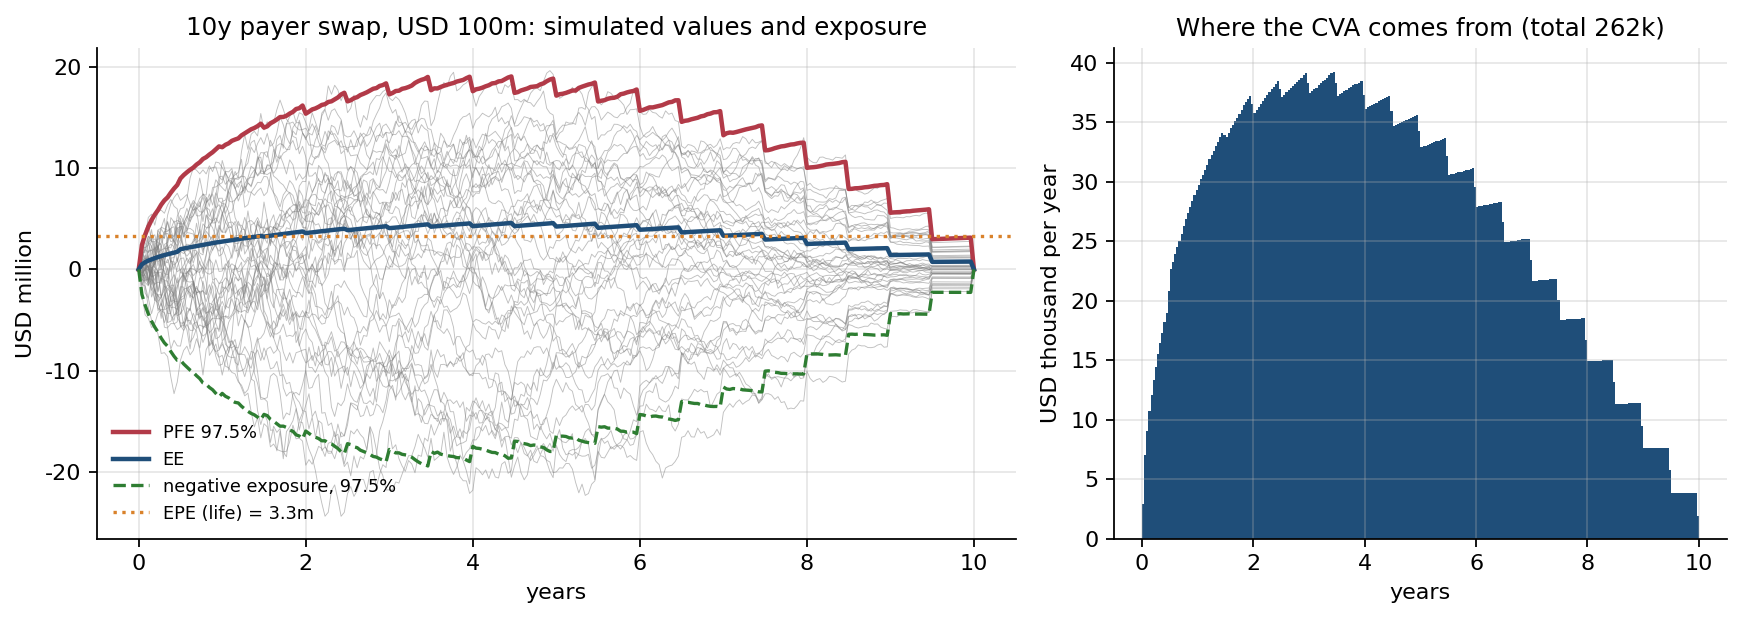
\includegraphics[width=\textwidth]{fig3_exposure.png}
\caption{Left: 40 simulated values of the 10-year payer swap, expected exposure (EE), 97.5\% potential future exposure (PFE) and 97.5\% negative exposure. Right: contribution of each date to the CVA, per year.}
\label{fig:exposure}
\end{figure}

Table~\ref{tab:cva} gives the main numbers. The unilateral CVA is USD 262{,}344 with a Monte Carlo standard error of 935 (0.4\%). Expressed as a running spread over the annuity of the swap, the bank should add about 3.4 bp a year to the fixed rate to be paid for the counterparty risk. The DVA, the symmetric benefit from the bank's own default risk, is USD 137{,}000; the bilateral CVA net of DVA is USD 122{,}000.

\begin{table}[h]
\centering
\caption{Exposure and credit valuation adjustments of the 10-year USD 100m payer swap.}
\label{tab:cva}
\begin{tabular}{lr}
\toprule
Measure & Value \\
\midrule
Par fixed rate & 5.100\% \\
Peak EE (at 4.5 years) & USD 4.59m \\
Peak PFE 97.5\% (at 4.5 years) & USD 19.09m \\
EPE over the life of the trade & USD 3.26m \\
Effective EPE over one year (Basel) & USD 1.80m \\
\midrule
Unilateral CVA (BBB, $\lambda=1.92\%$, LGD 60\%) & USD 262{,}344 \\
\quad Monte Carlo standard error & USD 935 \\
\quad in bp of notional / running bp per year & 26.2 / 3.4 \\
Unilateral DVA (A, $\lambda=1.27\%$) & USD 137{,}428 \\
Bilateral CVA / DVA (first to default) & USD 248{,}747 / 127{,}180 \\
Bilateral CVA $-$ DVA & USD 121{,}568 \\
\bottomrule
\end{tabular}
\end{table}

\paragraph{Sensitivities.} The CVA is close to proportional to the hazard rate (USD 137{,}000 with half the spread, 484{,}000 with twice the spread), because the default probabilities are small. It is less than proportional to the rate volatility: with $\sigma$ halved the CVA is USD 148{,}000 and with $\sigma \times 1.5$ it is 377{,}000. Part of the exposure comes from the drift of the forward curve, which does not depend on $\sigma$. The CVA of the receiver swap is lower, USD 203{,}000, because the upward-sloping curve makes the payer swap more likely to be in the money.

\subsection{Is the Monte Carlo right?}

Table~\ref{tab:checks} lists the checks, all of which are also automated in 23 unit tests. The most useful one uses a closed form. At a reset date $T_k$, the discounted positive value of the remaining swap is exactly the payoff of a payer swaption expiring at $T_k$, so $\text{EE}^*(T_k)$ must equal the swaption price. In Hull--White, this price is known in closed form \citep{jamshidian1989}: the swaption is a put on a coupon bond, which splits into a sum of zero-coupon bond puts. Figure~\ref{fig:swaption} compares both at the 19 reset dates: the largest relative error is 1.5\% and the largest gap is 2.35 standard errors, as expected from Monte Carlo noise. On a semi-annual grid, the CVA computed with the closed-form EE (USD 248{,}378) and with the Monte Carlo EE (248{,}651) differ by 0.1\%.

\begin{table}[h]
\centering
\caption{Consistency checks.}
\label{tab:checks}
\begin{tabular}{lr}
\toprule
Check & Result \\
\midrule
Bootstrap: par bonds repriced & error $< 10^{-15}$ \\
Swap value at $t=0$ (curve and every path) & 0 \\
$\mathbb{E}[D(t)]$ vs $P(0,t)$, all dates & max error 0.026\% \\
$\mathbb{E}[D(t)V(t)]$ vs forward swap value (reset dates) & max gap USD 13{,}800 (1.4 bp) \\
$\text{EE}^*(T_k)$ vs Jamshidian swaption, 19 dates & max error 1.5\%, max $|z|$ = 2.35 \\
CVA on a semi-annual grid, closed form vs MC & 248{,}378 vs 248{,}651 \\
Payer $-$ receiver swaption = forward swap & exact (unit test) \\
\bottomrule
\end{tabular}
\end{table}

\begin{figure}[h]
\centering
\begin{minipage}{0.49\textwidth}
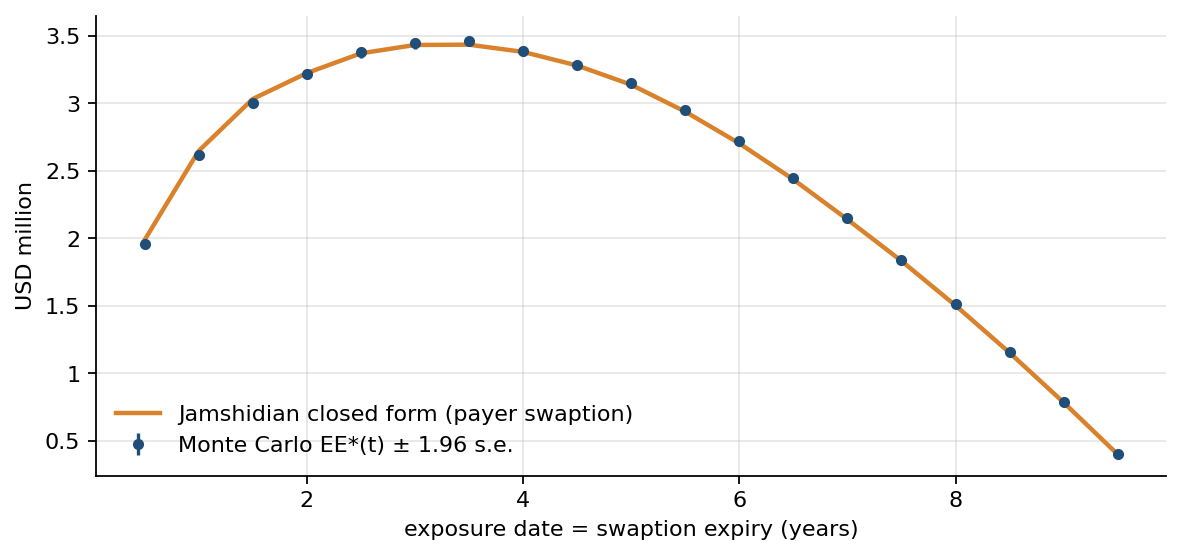
\includegraphics[width=\textwidth]{fig4_swaption_check.png}
\end{minipage}
\begin{minipage}{0.49\textwidth}
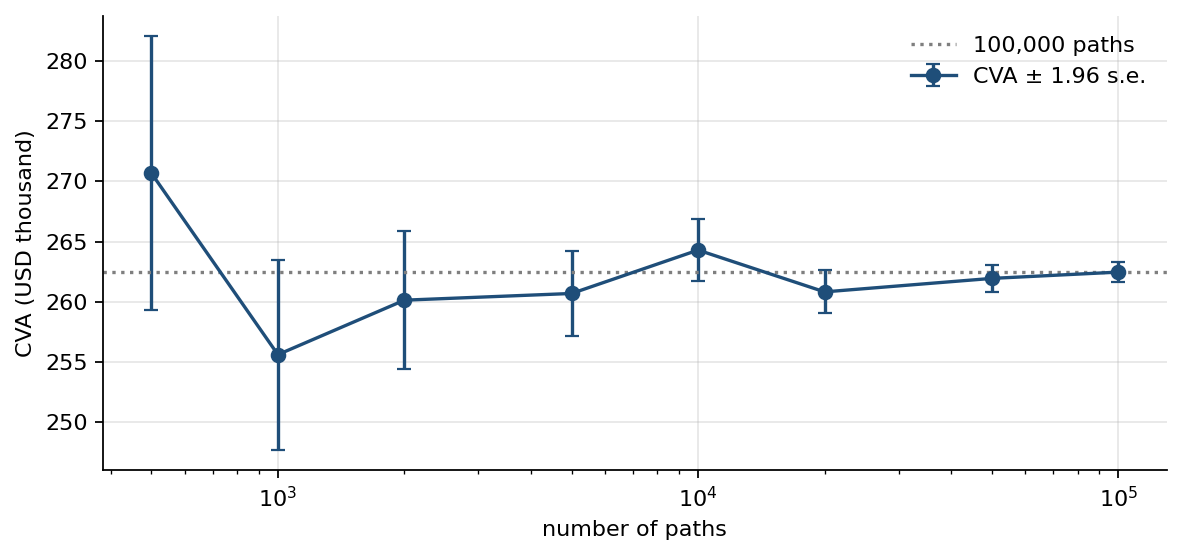
\includegraphics[width=\textwidth]{fig5_convergence.png}
\end{minipage}
\caption{Left: Monte Carlo discounted EE against the Jamshidian payer swaption price at each reset date. Right: CVA estimate and 95\% confidence interval against the number of paths (independent runs).}
\label{fig:swaption}
\end{figure}

\paragraph{Convergence.} Running the CVA again with independent random numbers and an increasing number of paths (Figure~\ref{fig:swaption}, right), the 95\% confidence interval shrinks from $\pm$11{,}400 with 500 paths to $\pm$800 with 100{,}000 paths, in line with the $1/\sqrt{N}$ rate \citep{glasserman2003}. The estimate with 100{,}000 paths (USD 262{,}458) differs from the base case by USD 114, about 0.1 of its standard error.

\subsection{Collateral}

Table~\ref{tab:csa} and Figure~\ref{fig:csa} show the effect of a two-way CSA. With daily, instantaneous margining and no threshold the exposure disappears. In reality, after a default the bank needs time to notice that collateral is missing, close out and replace the trade: the margin period of risk. With a 10-business-day MPR and a zero threshold, 10\% of the CVA remains (USD 27{,}000), and 15\% with 20 days. The threshold matters much more than the MPR: with a USD 5 million threshold, the CVA only falls by 38\%, whatever the MPR, because the bank remains unsecured up to the threshold, and the expected exposure of this trade is below USD 5 million most of the time. The peak PFE, however, is capped: from USD 19.1 million to 6.6 million. The small spikes of the collateralised profiles at coupon dates come from payments made during the MPR, a known effect \citep{gregory2020}.

\begin{table}[h]
\centering
\caption{CVA under a two-way CSA (USD, and share of the uncollateralised CVA of 262{,}344).}
\label{tab:csa}
\begin{tabular}{lrrrr}
\toprule
Threshold & \multicolumn{2}{c}{MPR 10 business days} & \multicolumn{2}{c}{MPR 20 business days} \\
 & CVA & share & CVA & share \\
\midrule
USD 10m & 232{,}363 & 88.6\% & 232{,}482 & 88.6\% \\
USD 5m & 163{,}185 & 62.2\% & 163{,}563 & 62.3\% \\
USD 2m & 81{,}680 & 31.1\% & 84{,}393 & 32.2\% \\
USD 1m & 48{,}914 & 18.6\% & 55{,}844 & 21.3\% \\
0 & 26{,}951 & 10.3\% & 38{,}664 & 14.7\% \\
\bottomrule
\end{tabular}
\end{table}

\begin{figure}[h]
\centering
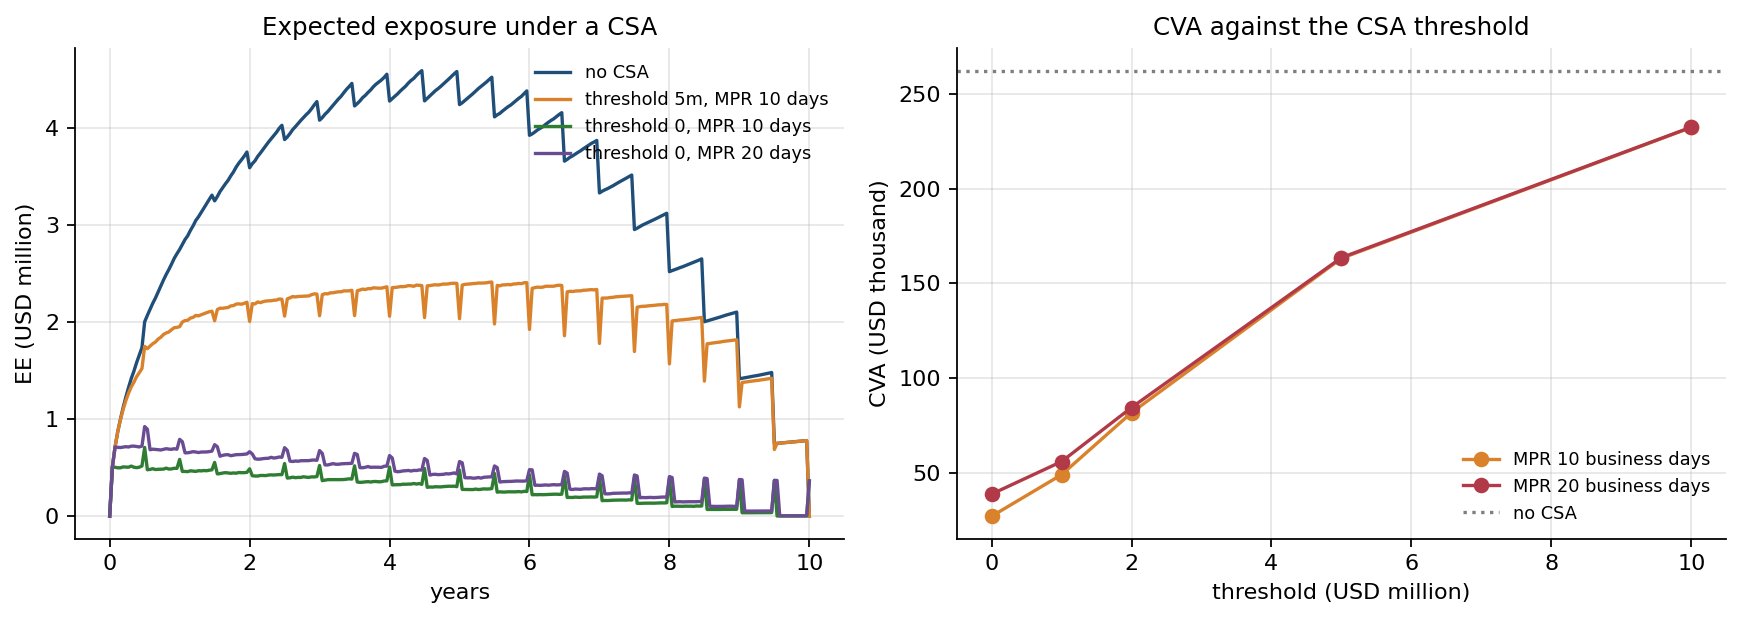
\includegraphics[width=\textwidth]{fig6_collateral.png}
\caption{Left: expected exposure without CSA and under three CSAs. Right: CVA against the threshold for two margin periods of risk.}
\label{fig:csa}
\end{figure}

\subsection{Netting}

If the client also has a 5-year receiver swap with the bank, the two trades offset each other over the first five years. Valued as one netting set, the combined CVA is USD 204{,}000 instead of 312{,}000 for the two trades taken separately: netting saves 35\% (Figure~\ref{fig:netting}). The peak of the summed standalone PFE profiles is USD 25.4 million; the peak PFE of the netting set is USD 18.5 million. If the second trade is a 5-year payer, netting saves nothing (0.03\%): in a one-factor model both trades gain value when rates rise, so their values almost never have opposite signs. A two-factor model, in which the 5- and 10-year rates do not move perfectly together, would give a small benefit.

\begin{figure}[h]
\centering
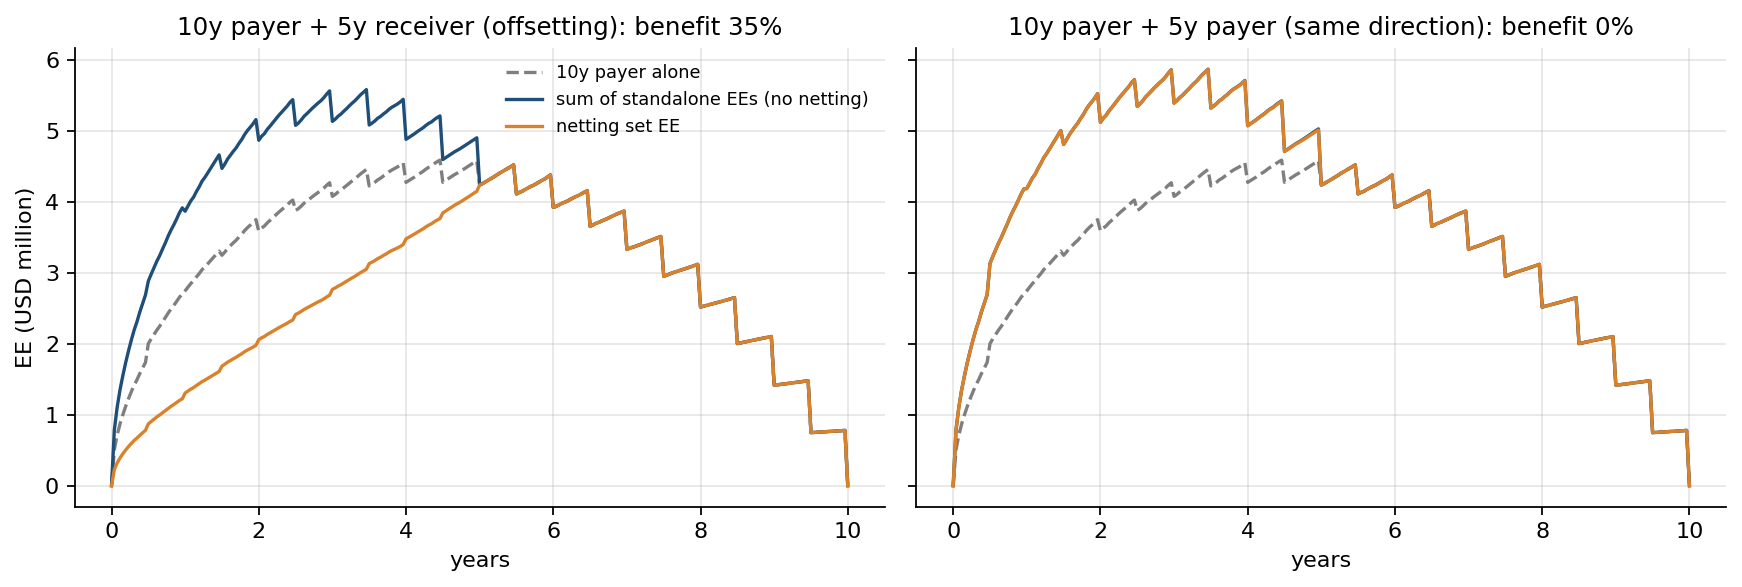
\includegraphics[width=\textwidth]{fig7_netting.png}
\caption{Expected exposure of the 10-year payer swap netted with a 5-year receiver (left) or a 5-year payer (right), against the sum of the standalone expected exposures.}
\label{fig:netting}
\end{figure}

\subsection{Wrong-way risk}

Figure~\ref{fig:wwr} and Table~\ref{tab:wwr} show the CVA when the default intensity of the counterparty is correlated with interest rates, with the default probabilities held on the market curve. At zero correlation the path-wise CVA equals the independent CVA up to Monte Carlo noise (ratio 1.00 to 1.01). With an intensity volatility of 50\%, a correlation of $+0.6$ raises the CVA of the payer swap by 55\% and a correlation of $+0.9$ by 85\%; negative correlation (right-way risk) lowers it. The receiver swap shows the mirror image. The effect grows with the volatility of the intensity: at $\rho=+0.9$ the CVA is multiplied by 1.41 with $\eta=25\%$ and by 2.62 with $\eta=100\%$.

A realistic wrong-way case for the bank's payer swap is a leveraged client that has swapped its fixed-rate bond into floating: the client pays floating, and both its swap payments and its other floating-rate debt grow when rates rise, exactly when the bank's exposure is largest. The opposite case is a client that pays fixed to hedge a floating-rate loan: the bank receives fixed, its exposure is largest when rates fall, while the client is hurt when rates rise, which is right-way risk. Which side is wrong-way depends on the client's business, so the sign of $\rho$ has to be argued trade by trade \citep{hullwhite2012wwr}.

\begin{figure}[h]
\centering
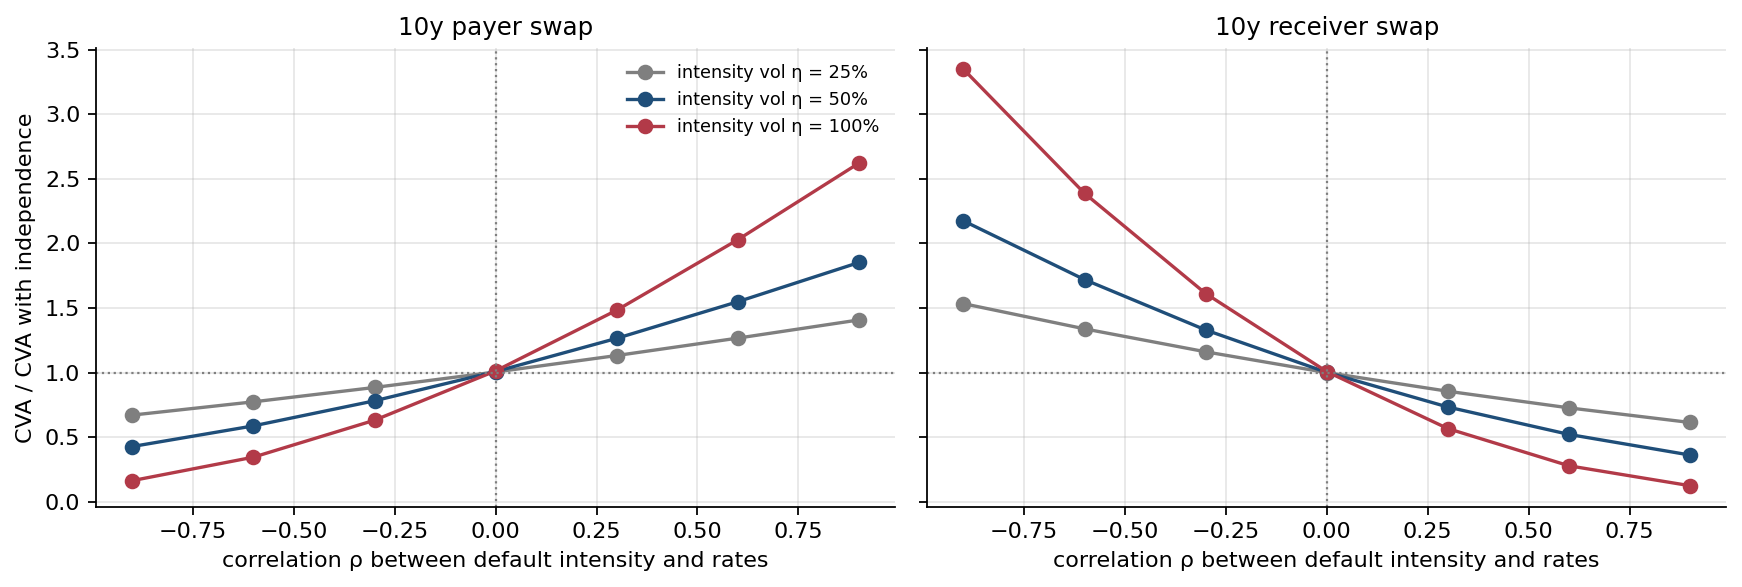
\includegraphics[width=\textwidth]{fig8_wrong_way_risk.png}
\caption{CVA with stochastic default intensity correlated with rates, relative to the CVA with independence, for the 10-year payer (left) and receiver (right) swaps.}
\label{fig:wwr}
\end{figure}

\begin{table}[h]
\centering
\caption{Payer-swap CVA relative to independence, by correlation $\rho$ and intensity volatility $\eta$.}
\label{tab:wwr}
\begin{tabular}{lrrrrrrr}
\toprule
$\rho$ & $-0.9$ & $-0.6$ & $-0.3$ & $0$ & $+0.3$ & $+0.6$ & $+0.9$ \\
\midrule
$\eta=25\%$ & 0.67 & 0.77 & 0.88 & 1.00 & 1.13 & 1.27 & 1.41 \\
$\eta=50\%$ & 0.43 & 0.59 & 0.78 & 1.01 & 1.26 & 1.55 & 1.85 \\
$\eta=100\%$ & 0.16 & 0.34 & 0.63 & 1.01 & 1.48 & 2.03 & 2.62 \\
\bottomrule
\end{tabular}
\end{table}

\section{Limitations}
\label{sec:limits}

\begin{itemize}
  \item \textbf{Curve.} The swap is priced on the Treasury curve with a single curve, because SOFR swap rates are not free. A real USD swap is projected and discounted on the SOFR curve; the swap spread is ignored. The par rate is therefore the Treasury par yield, not the market swap rate.
  \item \textbf{Volatility.} $a$ and $\sigma$ match historical (real-world) yield volatility, not swaption implied volatility, which a desk would use for pricing. A one-factor model cannot reproduce the hump of the volatility curve, nor imperfect correlation between maturities (hence no netting benefit between two payer swaps).
  \item \textbf{Credit.} A flat hazard rate from an index spread replaces the counterparty's own CDS curve; the LGD of 60\% is an assumption; the wrong-way-risk parameters $\kappa$ and $\eta$ are assumptions, so Section~4.5 is a sensitivity analysis.
  \item \textbf{Contract details.} The CSA ignores minimum transfer amounts, independent amounts, initial margin and collateral in securities; accruals are exactly 0.5 with no business-day calendar; funding (FVA) and capital (KVA) costs are left out.
\end{itemize}

\section{Conclusion}

From free data only, this project computes the CVA of a 10-year payer swap with a BBB counterparty in a Hull--White model fitted exactly to the Treasury curve: about USD 262{,}000 on USD 100 million, or 3.4 bp a year. The simulation is validated against the closed-form swaption price at every reset date. A CSA with a short margin period of risk removes most of the CVA, but the threshold matters more than the MPR, and netting helps only for trades that offset each other. Wrong-way risk can raise the CVA by half or more for plausible correlations. Natural extensions are a SOFR multi-curve set-up, a two-factor model calibrated to swaption volatilities, initial margin under SIMM, and the CVA capital charge under the Basel standardised approach \citep{basel2014,basel2017}.

\bibliographystyle{plainnat}
\bibliography{references}

\section*{Reproducibility}
All code, data and results are in the project repository. \texttt{python run\_all.py} recomputes every number and figure of this report from the saved FRED snapshot and runs the 23 unit tests; \texttt{python run\_all.py --download} downloads fresh data first.

\end{document}
